%!TeX root = ../main.tex
\section*{Lecture 16, 22/03/2018}
Today: More about the BRST-BV formalism.
Recall that we made a choice of generating set $G$ of symmetries giving the Noether identities.
These can be written as
\[
\delta \phi^i = \lambda^\alpha(\phi) R_\alpha^i + M^{ij} \frac{\delta S_0}{\delta \phi^j}
\]
for some antisymmetric matrix $M^{ij}$.
Notice that here the $R_\alpha^i$ are in $G$.

The bracket of $R_\alpha^i$ and $R_\beta^j$ is a gauge transformation, so it must be expressible as
\[
R_\alpha^j \frac{\delta R_\beta^i}{\delta \phi^j} - R_\beta^j \frac{\delta R_\alpha^i}{\delta \phi^j} = C_{\alpha \beta}^{\phantom{\alpha \beta} \gamma}(\phi) R_\gamma^i + M_{\alpha \beta}^{ij}(f) \frac{\delta S_0}{\delta \phi^j}.
\]
The case where $M_{\alpha \beta}^ij$ is nonzero is when we get an open algebra of symmetries.
$G$ is \emph{reducible} if there are $\lambda^\alpha$ such that
\[
\lambda^\alpha R_\alpha^i = N^{ij} \frac{\delta S_0}{\delta \phi^j},
\]
for $N^{ij}$ antisymmetric, and \emph{irreducible} otherwise.

Example: Consider topological Yang-Mills, with symmetries $\delta A_\mu^a = \varepsilon_\mu^a(x) + D_\mu f^a(x)$.
The first (topological) terms gives ghosts $\psi_\mu^a(x)$, while the second (gauge) term gives $c^a(x)$.
These are redundant via $\varepsilon_\mu = -D_\mu f$.
We could try to eliminate them but this would not really be desirable.
\me{Maybe something to do with ghosts-for-ghosts?}

Recall that in Hamiltonian quantum mechanics with a phase space $\Phi$, observables are just $C^\infty(\Phi)$.
In QFT, Lorentz symmetry messes up the choice of time direction, so to generalize this approach we'll have to do something different.
One idea is to view a point $(p,q)$ as initial conditions for some solutions to the equations of motion.
If we have a nondegenerate Hamiltonian, there will be a one-to-one correspondence between such points and solutions of the equations of motion.
We therefore \emph{define} covariant phase space $\Sigma$ to be the set of all covariant solutions to the equations of motion.
(See Figure \ref{fig:phase-space}.)

\begin{figure}[h]
\centering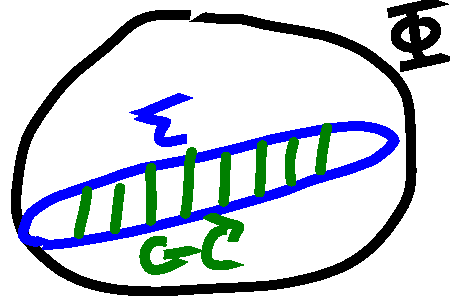
\includegraphics{fig/phase-space.pdf}
\caption{A diagram of various phase-space reductions.}
\label{fig:phase-space}
\end{figure}

We can write $C^\infty(\Sigma) = C^\infty(\Phi)/\mathfrak{N}$, where $\mathfrak N$ is the ideal of functions vanishing on $\Sigma$.
We want to identify this as the cohomology $H^0(\delta)$ of some differential.
The easiest way to do this is by introducing an antifield $\phi_i^*$ for each field $\phi^i$ and declaring
\begin{align*}
\delta \phi^i &= 0\\
\delta \phi_i^* &= -\frac{\delta S_0}{\delta \phi^i}.
\end{align*}
(This is the Koszul-Tate construction.)
Notice that these antifields don't have anything to do with gauge symmetry.
We also introduce a quantum number \me{i.e.~grading} called the antighost number, which is $0$ for fields and $-1$ for antifields.
We will later identify this with minus the ghost number.

A reasonable question at this point is: What about $H^p(\delta)$ for $p > 0$?
It will create problems, but it occurs (also other times) when there is gauge symmetry: If we have a Noether identity
\[
\frac{\delta S_0}{\delta \phi^i} R_\alpha^i = 0,
\]
then
\[
\delta\left(R_\alpha^i \phi_i^* \right) = 0,
\]
but it isn't $\delta$ of anything, so we get a nontrivial class in $H^1(\delta)$.

To fix this problem, we can add a $\phi_\alpha^*$ with $\delta \phi_\alpha^* = R_\alpha^i \phi_i^*$.
Now there is a potential obstacle at ghost number $2$, and if there's more reducibility we might need to keep repeating this process, requiring more and more antifields.
This has something to do with derived categories/geometry.

It can be shown that for a generic gauge theory, $\Sigma$ splits nicely into gauge orbits: there's an integrability condition on the action of $G$.
In particular, we can assume that $\Sigma$ is a $G$-fibration over our desired gauge-invariant phase space $\Sigma/G$.
(Again, see Figure \ref{fig:phase-space}.)
This reduction is just BRST again!

Define \emph{vertical vectors} to be vectors on $\Sigma$ tangent to the $G$-orbits, and similarly for vertical $p$-forms.
Then we can define $d$ by (arguments vertical vectors)
\begin{align*}
dF(X) &= \frac{\delta}{\delta X}F\\
d \alpha(X,Y) &= 0 - \mathcal{L}_Y \alpha(x) + \mathcal{L}_X \alpha(Y) + \alpha([X,Y]),
\end{align*}
and this will be the BRST charge.

Choose a basis of vertical vectors so that
\begin{align*}
X_\alpha F &= \frac{\delta F}{\delta \phi^i} R_\alpha^i\\
[X_\alpha, X_\beta] &= C_{\alpha \beta}^{\phantom{\alpha \beta} \gamma}(\phi) X_\gamma
\end{align*}
on $\Sigma$.
Introduce a basis $c^\alpha$ dual to $X_\alpha$, and define
\begin{align*}
dF &= (X_a F)c^\alpha\\
dc^\alpha &= \frac{1}{2} C_{\alpha \beta}^{\phantom{\alpha \beta} \gamma} c^\beta c^\gamma,
\end{align*}
which again is exactly the BRST charge action on the ghosts.

We now want to combine $\delta$ and $d$ together to a single operator $s$, but since $d \delta + \delta d \ne 0$, we can't just add them.
Instead we need to use \emph{homological perturbation theory}, which is a difficult piece of mathematics.
Once you know that it works, there's a shortcut:
Introduce an \emph{antibracket}
\[
sA = (A,S) 
\]
for a new object $S$.
We define $(\phi^i, \phi_j^*) = \delta^i_j$, $(c^\beta, \phi_\alpha^*) = \delta_\alpha^\beta$, etc.
The antibracket satisfies:
\begin{enumerate}
    \item $\operatorname{gh}\#(A,B) = \operatorname{gh}\# A + \operatorname{gh}\# B + 1$
    \item Parity $\epsilon(A,B)$ of $(A,B)$ is $\epsilon A + \epsilon B + 1$
    \item $(A,B) = (-1)^{(\epsilon A +1)(\epsilon B +1)}(B,A)$
    \item Super-Jacobi identity
\end{enumerate}
and if we choose $S$ so that $\operatorname{gh} \# S = 0$, $\epsilon S = 0$, $(S,S) =0$, then it will preserve the cohomology.

These requirements are the \emph{master equation}, and the solution will be
\[
S = \sum_{m \ge 0} S^{(m)}.
\]
Facts about $S$:
\begin{itemize}
    \item $S^{(0)}$ is just the action
    \item $(\phi_i^*,S(\phi_i)) = \delta \phi_i^*$
    \item $S^{(1)} = \phi_i^* R_\alpha^i c^\alpha$
\end{itemize}

The next step is gauge-fixing.
We have antighosts $b_A, B_A; b_A^*, B_A^*$.
We write our fields more compactly as $\phi^{\mathfrak{A}} = (\phi^i, c^\alpha, b_A, B_A)$ and $\phi_{\mathfrak{A}}^* = (\phi_i^*, \dots)$, which we can even combine together as $\mathcal{Z}^{\mathfrak{A}} = (\phi^{\mathfrak{A}}, \phi_{\mathfrak{B}}^*)$.
Here $\mathfrak{A}$ can take $2N$ values.
The antibracket is
\[
(A,B) = \frac{\delta^R A}{\delta \mathcal{Z}^{\mathfrak{A}}} \zeta^{\mathfrak{AB}} \frac{\delta^L B}{\delta \mathcal{Z}^{\mathfrak{B}}},
\]
where $\zeta^{\mathfrak{AB}}$ is just the standard symplectic matrix in the Fraktur indices.

We will therefore want to choose $N$ gauge-fixing conditions $\Omega^{\mathfrak{A}}(\mathcal{Z}) = 0$, which will need to satisfy $(\Omega^\mathfrak{A}, \Omega^\mathfrak{B}) = 0$ to make things work.